\documentclass[12pt,a4paper]{article}
\usepackage[utf8]{vietnam}
\usepackage{amsmath,amssymb}
\usepackage{tabularx}
\usepackage{tikz}
\usetikzlibrary{calc,angles,quotes,arrows.meta}
\usepackage{xcolor}
\usepackage{enumitem}
\usepackage{fancyhdr}
\usepackage[top=1.0cm, bottom=1.1cm, left=1.3cm, right=1.3cm]{geometry}
\usepackage[dethi]{ex_test}
\SAOPTN{widthSA=3.2,heightSA=0.62}

\setlength{\headheight}{15pt}
\setlength{\parskip}{1.5pt}

\pagestyle{fancy}
\fancyhf{}
\lhead{\textit{Trường THCS Sơn Tây -- Đề KSCL Lớp 9 Lần 1 (2026 -- 2027)}}
\rhead{\textit{Mã đề: 02 -- Môn Toán}}
\cfoot{\thepage/2}

\begin{document}

% =============================================================================
% TRANG 1: TIÊU ĐỀ & PHẦN I TRẮC NGHIỆM
% =============================================================================
\noindent
\begin{tabularx}{\linewidth}{X r}
  \textbf{TRƯỜNG THCS SƠN TÂY} & \textbf{ĐỀ KHẢO SÁT CHẤT LƯỢNG LỚP 9 -- LẦN 1} \\
  \textbf{NĂM HỌC 2026 -- 2027} & \textbf{MÔN: TOÁN} \\
  \textbf{MÃ ĐỀ: 02} \textit{(Đề thi gồm 02 trang)} & \textit{Thời gian làm bài: 90 phút (không kể thời gian giao đề)} \\
\end{tabularx}
\vspace{-1mm}
\hrule
\vspace{2mm}

\noindent\textbf{Họ và tên thí sinh:} \dotfill \textbf{Lớp:} \dotfill \textbf{SBD:} \dotfill

\vspace{2mm}
\noindent\textbf{\large PHẦN I. TRẮC NGHIỆM KHÁCH QUAN (2,0 điểm)}

\noindent\textit{Học sinh trả lời từ Câu 1 đến Câu 8. Mỗi câu hỏi chỉ chọn một phương án đúng duy nhất và ghi chữ cái đứng trước phương án đó vào bảng trả lời bên dưới.}

\vspace{1.5mm}
\begin{center}
\renewcommand{\arraystretch}{1.25}
\begin{tabular}{|c|c|c|c|c|c|c|c|c|}
\hline
\textbf{Câu} & \textbf{1} & \textbf{2} & \textbf{3} & \textbf{4} & \textbf{5} & \textbf{6} & \textbf{7} & \textbf{8} \\
\hline
\textbf{Đáp án} & \hspace{1.1cm} & \hspace{1.1cm} & \hspace{1.1cm} & \hspace{1.1cm} & \hspace{1.1cm} & \hspace{1.1cm} & \hspace{1.1cm} & \hspace{1.1cm} \\
\hline
\end{tabular}
\end{center}
\vspace{1.5mm}

\begin{enumerate}[label=\textbf{Câu \arabic*.}, leftmargin=*, itemsep=4.5pt, parsep=0pt]
  \item Phương trình nào sau đây là phương trình bậc nhất hai ẩn?
  \begin{flushleft}
    \begin{tabularx}{\linewidth}{X X X X}
      \textbf{A.} $0x + 0y = 3$ & 
      \textbf{B.} $3x + y = 0$ & 
      \textbf{C.} $x - 3\sqrt{y} = 5$ & 
      \textbf{D.} $x + \dfrac{2}{y} = 1$
    \end{tabularx}
  \end{flushleft}

  \item Nghiệm của phương trình $3x + 4 = 1$ là
  \begin{flushleft}
    \begin{tabularx}{\linewidth}{X X X X}
      \textbf{A.} $1$ & 
      \textbf{B.} $-2$ & 
      \textbf{C.} $2$ & 
      \textbf{D.} $-1$
    \end{tabularx}
  \end{flushleft}

  \item Cặp số nào dưới đây là nghiệm của phương trình $x + 3y = 5$?
  \begin{flushleft}
    \begin{tabularx}{\linewidth}{X X X X}
      \textbf{A.} $(2; 1)$ & 
      \textbf{B.} $(1; 2)$ & 
      \textbf{C.} $(-1; -2)$ & 
      \textbf{D.} $(-2; -1)$
    \end{tabularx}
  \end{flushleft}

  \item Cặp số $(-2; 3)$ là nghiệm của hệ phương trình nào dưới đây?
  \begin{flushleft}
    \begin{tabularx}{\linewidth}{X X X X}
      \textbf{A.} $\begin{cases} 2x + y = 1 \\ 5x - y = 5 \end{cases}$ & 
      \textbf{B.} $\begin{cases} 3x + 2y = 1 \\ x - y = 6 \end{cases}$ & 
      \textbf{C.} $\begin{cases} x + y = 1 \\ x - 3y = -11 \end{cases}$ & 
      \textbf{D.} $\begin{cases} x + y = -5 \\ -x - 2y = 6 \end{cases}$
    \end{tabularx}
  \end{flushleft}

  \item Nghiệm của bất phương trình $x + 6 \le 0$ là:
  \begin{flushleft}
    \begin{tabularx}{\linewidth}{X X X X}
      \textbf{A.} $x < 6$ & 
      \textbf{B.} $x > -6$ & 
      \textbf{C.} $x \le 6$ & 
      \textbf{D.} $x \le -6$
    \end{tabularx}
  \end{flushleft}

  \item Cho đường tròn $(O; R)$. Điểm $M$ nằm bên trong đường tròn $(O; R)$ nếu:
  \begin{flushleft}
    \begin{tabularx}{\linewidth}{X X X X}
      \textbf{A.} $OM > R$ & 
      \textbf{B.} $OM = R$ & 
      \textbf{C.} $OM < R$ & 
      \textbf{D.} $OM \ge R$
    \end{tabularx}
  \end{flushleft}

  \item Cho $\Delta ABC$ vuông tại $A$, khi đó $\sin C$ bằng
  \begin{flushleft}
    \begin{tabularx}{\linewidth}{X X X X}
      \textbf{A.} $\dfrac{AB}{BC}$ & 
      \textbf{B.} $\dfrac{AC}{BC}$ & 
      \textbf{C.} $\dfrac{AC}{AB}$ & 
      \textbf{D.} $\dfrac{AB}{AC}$
    \end{tabularx}
  \end{flushleft}

  \item Cho $\Delta ABC$ vuông tại $A$ có $AB = 3\sqrt{3}\,\text{cm}$ và $AC = 3\,\text{cm}$. Khi đó số đo góc $C$ là
  \begin{flushleft}
    \begin{tabularx}{\linewidth}{X X X X}
      \textbf{A.} $90^\circ$ & 
      \textbf{B.} $30^\circ$ & 
      \textbf{C.} $60^\circ$ & 
      \textbf{D.} $45^\circ$
    \end{tabularx}
  \end{flushleft}
\end{enumerate}

\newpage

% =============================================================================
% TRANG 2: PHẦN II TỰ LUẬN
% =============================================================================
\noindent\textbf{\large PHẦN II. TỰ LUẬN (8,0 điểm)}

\begin{enumerate}[label=\textbf{Câu \arabic*.}, leftmargin=*, itemsep=4pt, parsep=0pt, start=9]
  \item \textbf{(2,0 điểm)} Giải các phương trình sau:
  \begin{enumerate}[label=\alph*), leftmargin=20pt, itemsep=2pt]
    \item $(2 - x)(2x + 1) = 0$
    \item $\dfrac{3}{x + 1} + \dfrac{2}{x - 3} = \dfrac{3}{(x + 1)(x - 3)}$
  \end{enumerate}

  \item \textbf{(1,0 điểm)} Giải hệ phương trình: $\begin{cases} x + 5y = -11 \\ 2x - 3y = 4 \end{cases}$

  \item \textbf{(1,0 điểm)} \textit{Giải bài toán sau bằng cách lập phương trình hoặc hệ phương trình:}
  
  Trong kỳ thi Tuyển sinh vào lớp 10 THPT năm học 2026 -- 2027, hai trường A và B có tổng cộng 385 học sinh dự thi. Kết quả là hai trường có tổng cộng 327 học sinh trúng tuyển, trong đó trường A có 90\% và trường B có 80\% học sinh dự thi trúng tuyển. Hỏi mỗi trường có bao nhiêu thí sinh dự thi?

  \item \textbf{(1,0 điểm)} 
  \par\noindent
  \begin{minipage}[t]{0.68\linewidth}
    Một cái cây có bóng trên mặt đất dài $40\,\text{m}$, biết rằng góc tạo bởi tia nắng mặt trời với mặt đất là $35^\circ$. Hỏi cái cây cao bao nhiêu mét? (kết quả làm tròn đến chữ số hàng đơn vị).
  \end{minipage}\hfill
  \begin{minipage}[t]{0.30\linewidth}
    \vspace{-2mm}
    \centering
    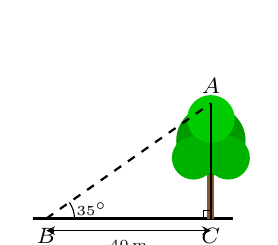
\begin{tikzpicture}[scale=0.55, >=stealth]
      \draw[thick] (-0.3,0) -- (4.3,0);
      \coordinate (C) at (3.8,0);
      \coordinate (B) at (0,0);
      \coordinate (A) at (3.8,2.66);
      
      \node[below] at (B) {\footnotesize $B$};
      \node[below] at (C) {\footnotesize $C$};
      \node[above] at (A) {\footnotesize $A$};
      
      % Thân cây và tán cây
      \draw[brown!70!black, line width=2.5pt] (3.8,0) -- (3.8,1.2);
      \fill[green!60!black] (3.8,1.8) circle (0.8);
      \fill[green!70!black] (3.4,1.4) circle (0.5);
      \fill[green!70!black] (4.2,1.4) circle (0.5);
      \fill[green!80!black] (3.8,2.3) circle (0.55);
      \draw[line width=1.0pt] (3.8,0) -- (3.8,2.66);
      
      % Tia nắng
      \draw[thick, dashed] (B) -- (A);
      
      % Góc vuông tại C
      \draw (C) ++(0,0.18) -- ++(-0.18,0) -- ++(0,-0.18);
      
      % Góc 35 độ tại B
      \draw (B) ++(0.65,0) arc (0:35:0.65);
      \node at (1.05,0.22) {\tiny $35^\circ$};
      
      \draw[<->] (0,-0.28) -- (3.8,-0.28);
      \node[below] at (1.9,-0.28) {\tiny $40\,\text{m}$};
    \end{tikzpicture}
  \end{minipage}

  \item \textbf{(2,0 điểm)} Cho tam giác $ABC$ vuông tại $A$, đường cao $AH$ ($H$ thuộc cạnh $BC$). Biết độ dài cạnh $AB = 6\,\text{cm}$, $AC = 8\,\text{cm}$.
  \begin{enumerate}[label=\alph*), leftmargin=20pt, itemsep=2pt]
    \item \textbf{(1,0 điểm)} Tính độ dài cạnh $BC$, đường cao $AH$ và số đo góc $B$ (số đo góc làm tròn đến độ).
    \item \textbf{(1,0 điểm)} Gọi $E$ và $F$ lần lượt là hình chiếu của $H$ trên cạnh $AB$ và $AC$. Chứng minh rằng: $AE \cdot AB = AF \cdot AC$ và tam giác $AEF$ đồng dạng với tam giác $ACB$.
  \end{enumerate}

  \item \textbf{(1,0 điểm)}
  \begin{enumerate}[label=\alph*), leftmargin=20pt, itemsep=2pt]
    \item \textbf{(0,5 điểm)} 
    \par\noindent
    \begin{minipage}[t]{0.70\linewidth}
      Một mảnh đất hình vuông có cạnh $30\,\text{m}$. Người ta xây dựng một vườn hoa hình vuông $EFGH$ có đỉnh $E, F, G, H$ lần lượt thuộc các cạnh của hình vuông $ABCD$ (như hình bên). Xác định vị trí điểm $E$ trên cạnh $AB$ để diện tích vườn hoa nhỏ nhất.
    \end{minipage}\hfill
    \begin{minipage}[t]{0.28\linewidth}
      \vspace{-2mm}
      \centering
      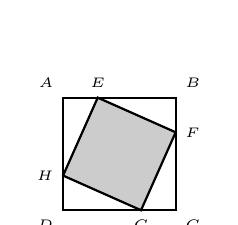
\begin{tikzpicture}[scale=0.55]
        \coordinate (A) at (0,2.6);
        \coordinate (B) at (2.6,2.6);
        \coordinate (C) at (2.6,0);
        \coordinate (D) at (0,0);
        
        \draw[thick] (A) -- (B) -- (C) -- (D) -- cycle;
        \node[above left] at (A) {\tiny $A$};
        \node[above right] at (B) {\tiny $B$};
        \node[below right] at (C) {\tiny $C$};
        \node[below left] at (D) {\tiny $D$};
        
        \coordinate (E) at (0.8,2.6);
        \coordinate (F) at (2.6,1.8);
        \coordinate (G) at (1.8,0);
        \coordinate (H) at (0,0.8);
        
        \fill[gray!40] (E) -- (F) -- (G) -- (H) -- cycle;
        \draw[thick] (E) -- (F) -- (G) -- (H) -- cycle;
        
        \node[above] at (E) {\tiny $E$};
        \node[right] at (F) {\tiny $F$};
        \node[below] at (G) {\tiny $G$};
        \node[left] at (H) {\tiny $H$};
      \end{tikzpicture}
    \end{minipage}

    \item \textbf{(0,5 điểm)} Cho các số thực $a, b$ thay đổi thoả mãn $a^2 + b^2 = 2$. Tìm giá trị nhỏ nhất của biểu thức $P = 3(a + b) + ab$.
  \end{enumerate}
\end{enumerate}

\vfill
\begin{center}
  \textbf{--- HẾT ---}\\
  \textit{\footnotesize Cán bộ coi thi không giải thích gì thêm.}
\end{center}

\end{document}

